% Options for packages loaded elsewhere
\PassOptionsToPackage{unicode}{hyperref}
\PassOptionsToPackage{hyphens}{url}
%
\documentclass[
]{book}
\usepackage{lmodern}
\usepackage{amssymb,amsmath}
\usepackage{ifxetex,ifluatex}
\ifnum 0\ifxetex 1\fi\ifluatex 1\fi=0 % if pdftex
  \usepackage[T1]{fontenc}
  \usepackage[utf8]{inputenc}
  \usepackage{textcomp} % provide euro and other symbols
\else % if luatex or xetex
  \usepackage{unicode-math}
  \defaultfontfeatures{Scale=MatchLowercase}
  \defaultfontfeatures[\rmfamily]{Ligatures=TeX,Scale=1}
\fi
% Use upquote if available, for straight quotes in verbatim environments
\IfFileExists{upquote.sty}{\usepackage{upquote}}{}
\IfFileExists{microtype.sty}{% use microtype if available
  \usepackage[]{microtype}
  \UseMicrotypeSet[protrusion]{basicmath} % disable protrusion for tt fonts
}{}
\makeatletter
\@ifundefined{KOMAClassName}{% if non-KOMA class
  \IfFileExists{parskip.sty}{%
    \usepackage{parskip}
  }{% else
    \setlength{\parindent}{0pt}
    \setlength{\parskip}{6pt plus 2pt minus 1pt}}
}{% if KOMA class
  \KOMAoptions{parskip=half}}
\makeatother
\usepackage{xcolor}
\IfFileExists{xurl.sty}{\usepackage{xurl}}{} % add URL line breaks if available
\IfFileExists{bookmark.sty}{\usepackage{bookmark}}{\usepackage{hyperref}}
\hypersetup{
  pdftitle={Photochemistry and Photophysics Workshop},
  pdfauthor={Fiona Dickinson},
  hidelinks,
  pdfcreator={LaTeX via pandoc}}
\urlstyle{same} % disable monospaced font for URLs
\usepackage{longtable,booktabs}
% Correct order of tables after \paragraph or \subparagraph
\usepackage{etoolbox}
\makeatletter
\patchcmd\longtable{\par}{\if@noskipsec\mbox{}\fi\par}{}{}
\makeatother
% Allow footnotes in longtable head/foot
\IfFileExists{footnotehyper.sty}{\usepackage{footnotehyper}}{\usepackage{footnote}}
\makesavenoteenv{longtable}
\usepackage{graphicx,grffile}
\makeatletter
\def\maxwidth{\ifdim\Gin@nat@width>\linewidth\linewidth\else\Gin@nat@width\fi}
\def\maxheight{\ifdim\Gin@nat@height>\textheight\textheight\else\Gin@nat@height\fi}
\makeatother
% Scale images if necessary, so that they will not overflow the page
% margins by default, and it is still possible to overwrite the defaults
% using explicit options in \includegraphics[width, height, ...]{}
\setkeys{Gin}{width=\maxwidth,height=\maxheight,keepaspectratio}
% Set default figure placement to htbp
\makeatletter
\def\fps@figure{htbp}
\makeatother
\setlength{\emergencystretch}{3em} % prevent overfull lines
\providecommand{\tightlist}{%
  \setlength{\itemsep}{0pt}\setlength{\parskip}{0pt}}
\setcounter{secnumdepth}{5}
\usepackage{booktabs}
\usepackage{amsthm}
\makeatletter
\def\thm@space@setup{%
  \thm@preskip=8pt plus 2pt minus 4pt
  \thm@postskip=\thm@preskip
}
\makeatother
\usepackage[]{natbib}
\bibliographystyle{apalike}

\title{Photochemistry and Photophysics Workshop}
\author{Fiona Dickinson}
\date{2020-10-29}

\begin{document}
\maketitle

{
\setcounter{tocdepth}{1}
\tableofcontents
}
\hypertarget{welcome}{%
\chapter*{Welcome}\label{welcome}}
\addcontentsline{toc}{chapter}{Welcome}

The notes have been prepared in a package called BookDown for RStudio so that the equations are accessible to screen readers. However, by providing the notes as a .html webpage I can also embed short videos to further describe some of the topics. Further you can download the questions (and later the answers, top left of the screen) in a format that suits you (either pdf or epub) to view offline, or change the way this document appears for ease of reading.

\hypertarget{workshops-for-photochemistry-photophysics}{%
\section*{Workshops for Photochemistry \& Photophysics}\label{workshops-for-photochemistry-photophysics}}
\addcontentsline{toc}{section}{Workshops for Photochemistry \& Photophysics}

This answerbook for CH30129 workshops will be updated weekly (hopefully the day after workshops) including thoughts and answers from you as a class. I will include video workthroughs of some answers, but others will be text based.

I am using this format as it is an accessible format.

\hypertarget{version-history}{%
\section*{Version history}\label{version-history}}
\addcontentsline{toc}{section}{Version history}

Week 6 questions 291020

Week 5 questions 201020

Week 4 questions 131020

Updated to correct type on question 3.2.2 121020

Updated to include workshop week 3 questions 091020

Updated to include workshop week 2 questions 021020

Typos on workshop 1 were fixed 280920

The initial commit of this book is dated 25th September 2020.

\hypertarget{ch:Workshop1}{%
\chapter{Workshop Questions for Week 1}\label{ch:Workshop1}}

\hypertarget{sec:BeerLambert}{%
\section{Short mathematical question - Beer Lambert law}\label{sec:BeerLambert}}

\begin{itemize}
\tightlist
\item
  How far can monochromatic 489 nm light travel through a 0.100 M solution of fluorescein with an extinction coefficient at 489 nm of 92000 M\textsuperscript{−1} cm\textsuperscript{−1} before 90 \% of it is absorbed?
  \emph{(I will use MCQs and UniDoodle to ask this in class)}
\end{itemize}

\hypertarget{sec:MolarExtinction}{%
\section{Short conceptual question - molar extinction coefficient}\label{sec:MolarExtinction}}

\begin{itemize}
\tightlist
\item
  Modify the molecule in figure \ref{fig:bpy} to increase the molar extinction coefficient (do not worry about what may happen to wavelength).
\end{itemize}

\begin{figure}

{\centering 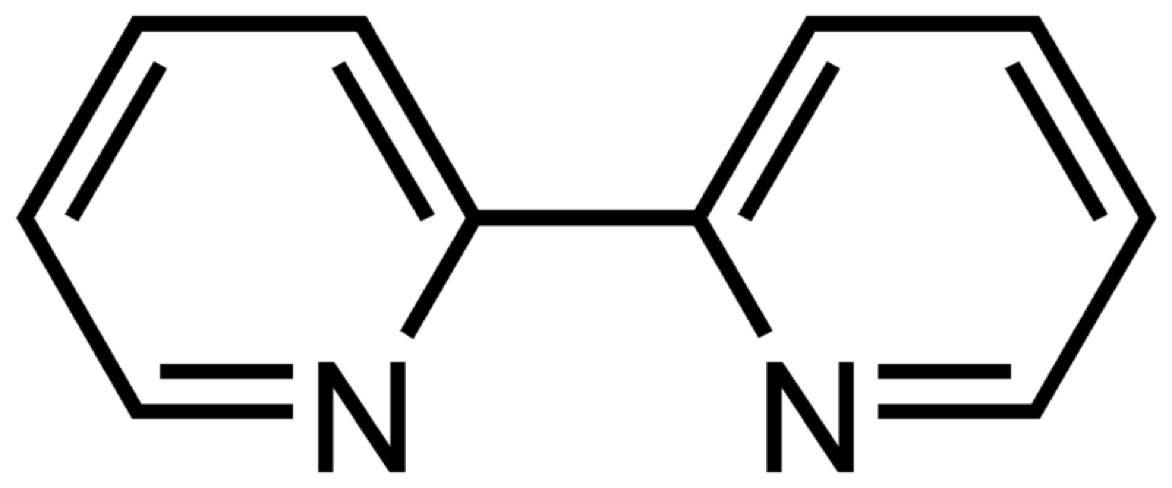
\includegraphics[width=0.3\linewidth]{images/bpy} 

}

\caption{The structure of bipyridine (also known as bpy).}\label{fig:bpy}
\end{figure}

\emph{(I will use UniDoodle's drawing feature to ask this in class)}

\hypertarget{sec:intensity}{%
\section{Short conceptual question - intensity of colour}\label{sec:intensity}}

\begin{itemize}
\tightlist
\item
  What factors influence the `intensity of colour' of the following solutions?
\end{itemize}

\begin{figure}

{\centering 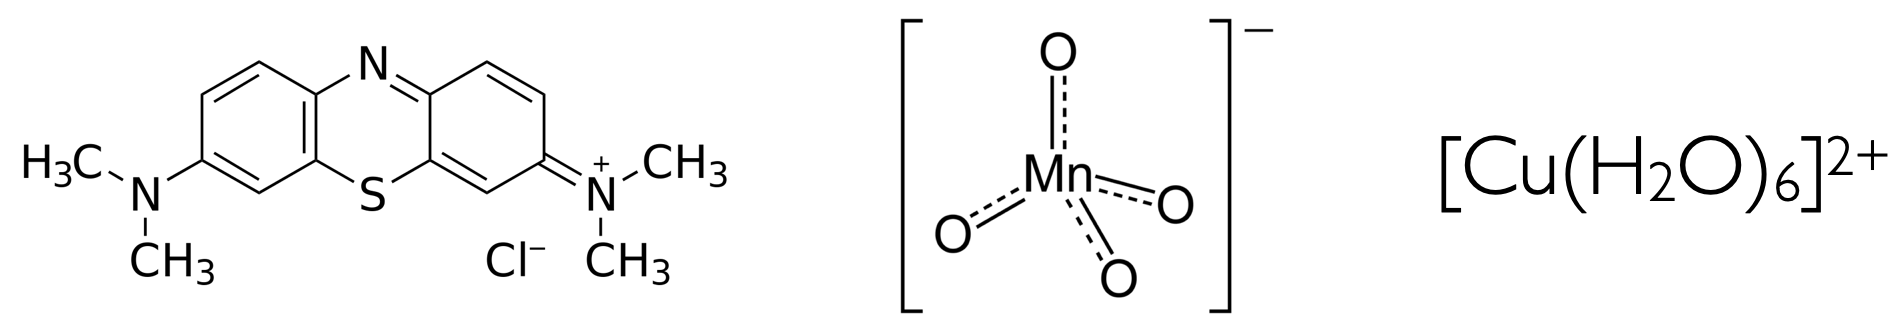
\includegraphics[width=0.7\linewidth]{images/molarextquestion} 

}

\caption{The structures of the organic dye methylene blue (left), potassium permanganate (centre) and copper hexa-aqua (right).}\label{fig:molarextstructures}
\end{figure}

\begin{figure}

{\centering 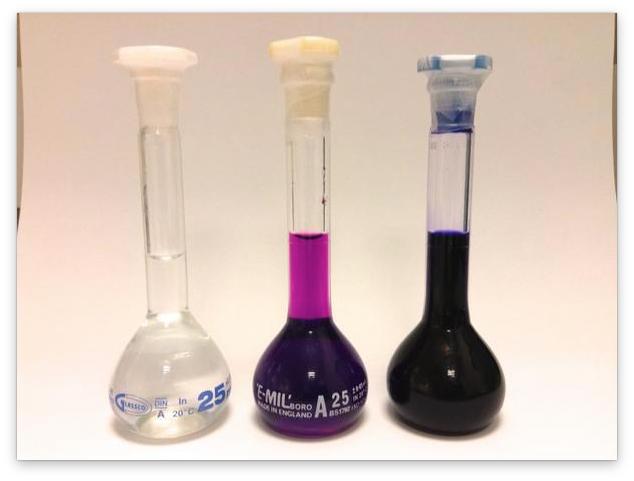
\includegraphics[width=0.7\linewidth]{images/Molar_extinction_coefficients} 

}

\caption{1 mM solutions of the organic dye methylene blue (right), potassium permanganate (centre) and copper hexa-aqua (left).}\label{fig:molarextsolutions}
\end{figure}

\emph{(This will be a discussion question - please feel free to raise a hand or write comments in the zoom chat)}

\hypertarget{sec:linewidth}{%
\section{Short conceptual question - line width}\label{sec:linewidth}}

\begin{itemize}
\tightlist
\item
  Why are some spectra very broad (figure \ref{fig:molecular}), whereas others have sharp peaks (figure \ref{fig:atomic})?
\end{itemize}

You will need to look at the x-scale to truley note the difference in the width of these emission spectra.

\begin{figure}

{\centering 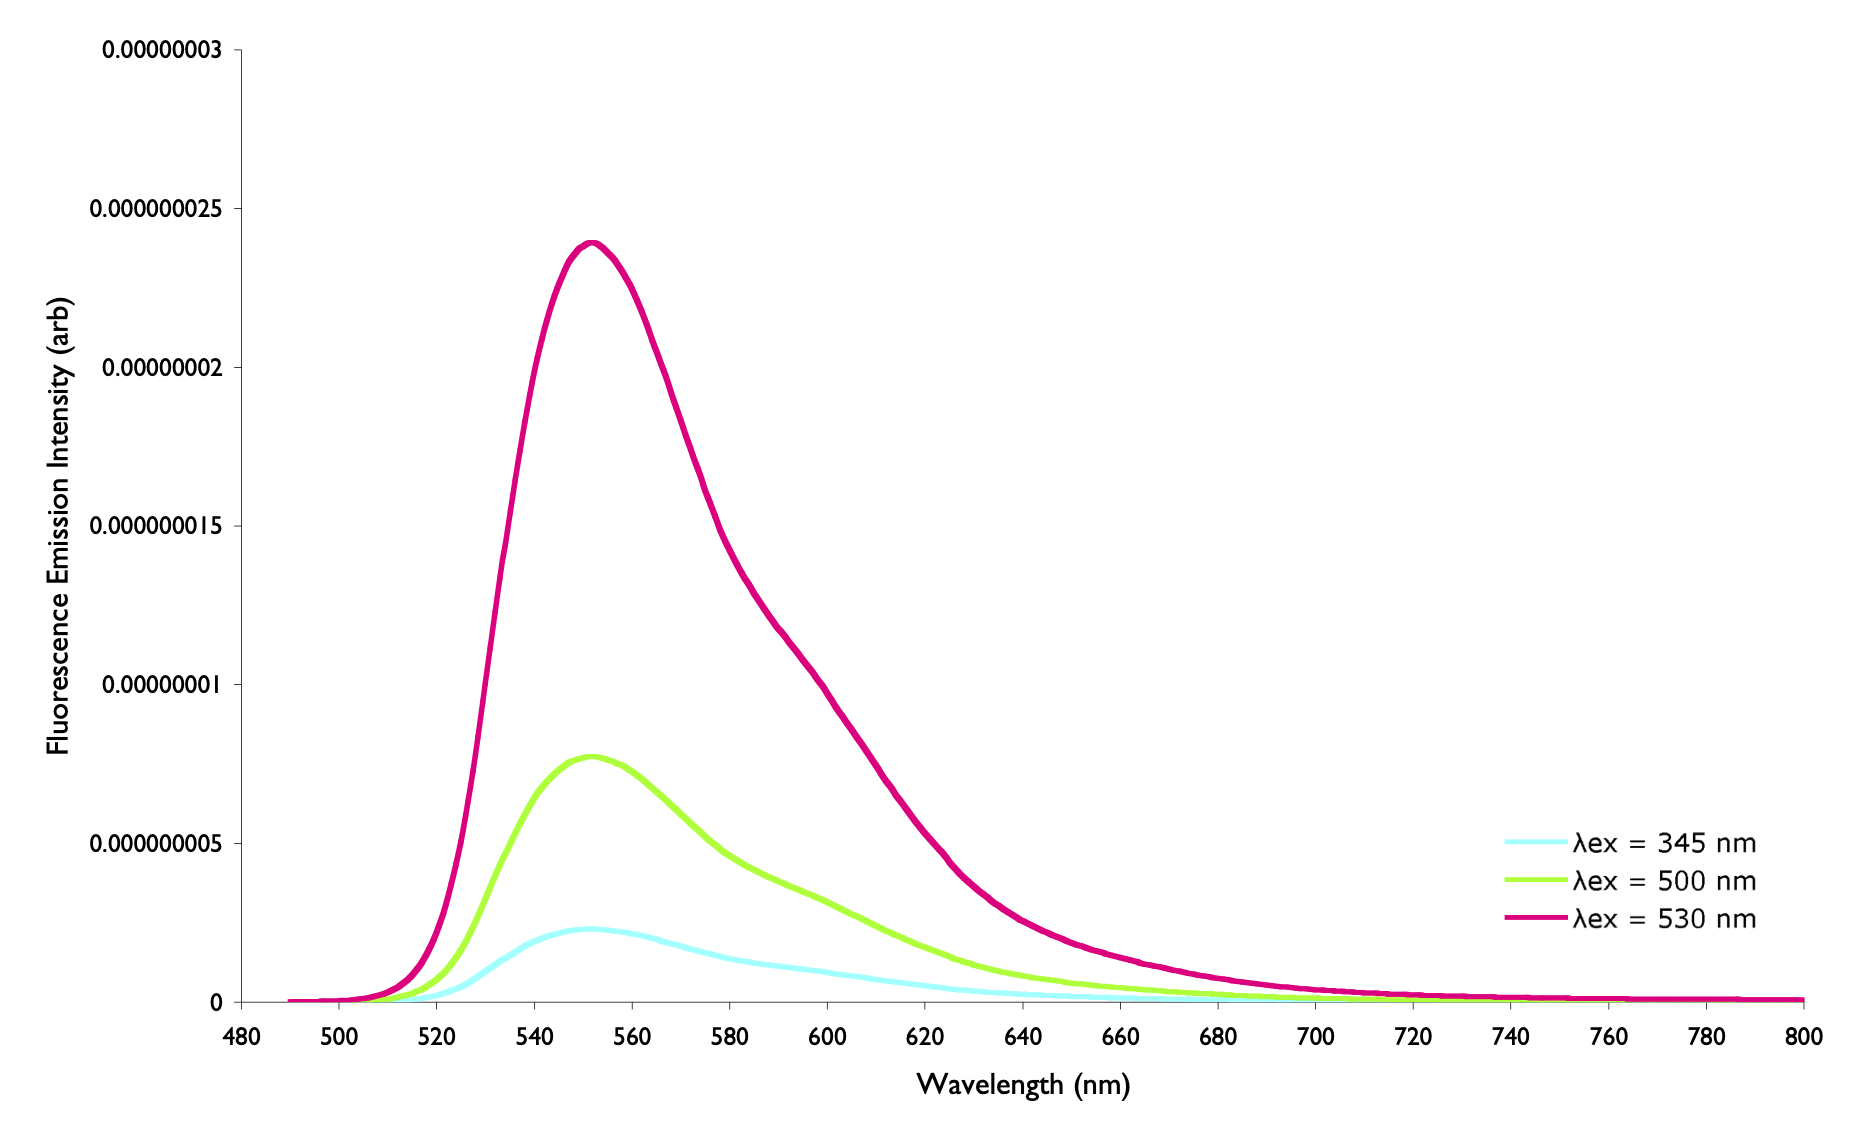
\includegraphics[width=0.7\linewidth]{images/rhodamine6G} 

}

\caption{The emission spectrum of rhodamine 6G}\label{fig:molecular}
\end{figure}

\begin{figure}

{\centering 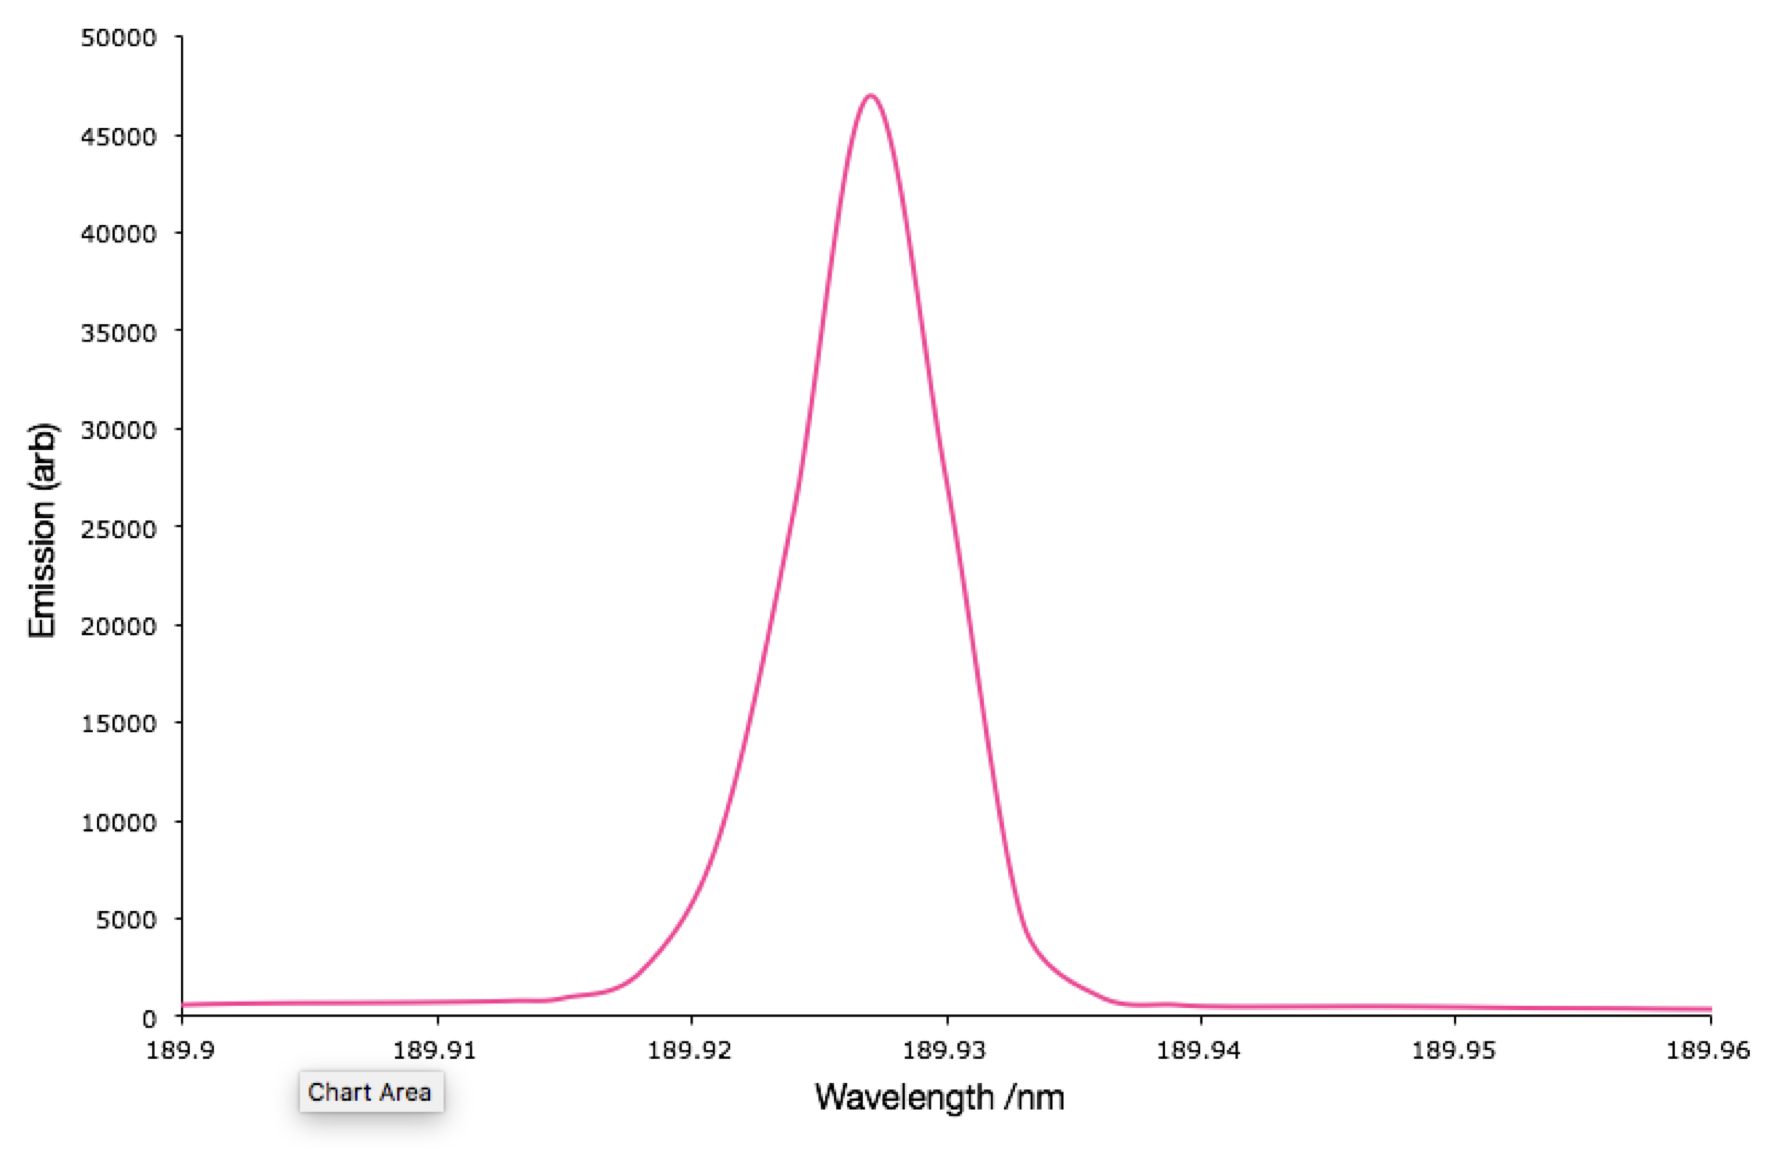
\includegraphics[width=0.7\linewidth]{images/atomic_emission_spectrum} 

}

\caption{The emission spectrum of Sn(II)}\label{fig:atomic}
\end{figure}

\emph{(This will be a discussion question - please feel free to raise a hand or write comments in the zoom chat)}

\hypertarget{sec:solvationabs}{%
\section{Short conceptual question - the effect of solvation on absorbance}\label{sec:solvationabs}}

\begin{figure}

{\centering 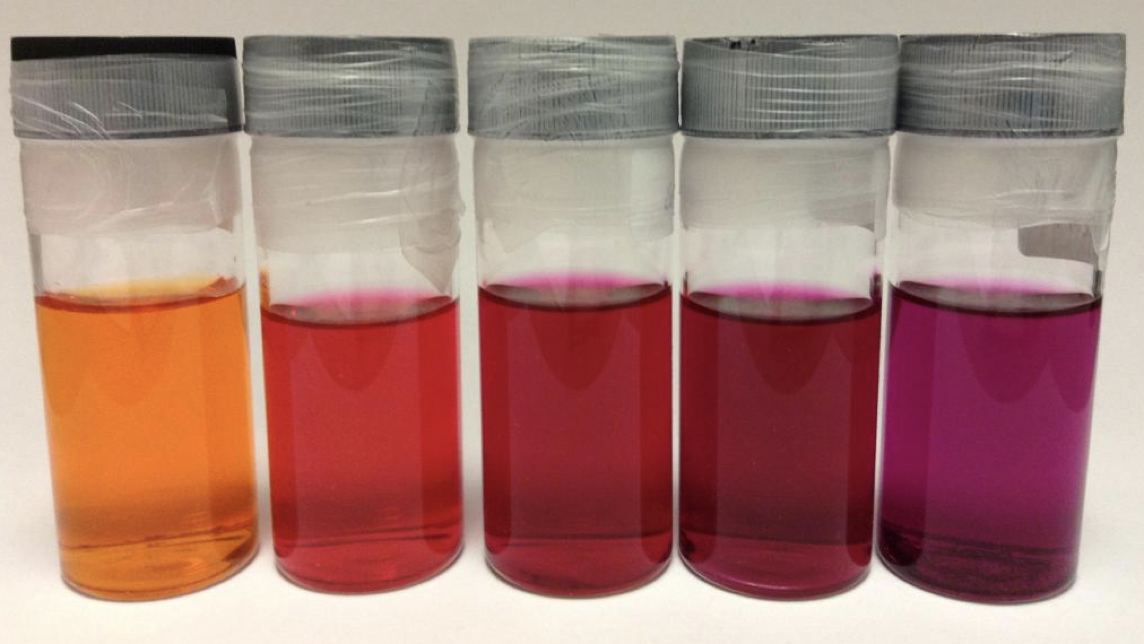
\includegraphics[width=0.7\linewidth]{images/ethidium} 

}

\caption{Ethidium bromide dissolved in from right; water(orange), methanol, ethanol, propanol and butanol(purple)}\label{fig:ethidium}
\end{figure}

\begin{itemize}
\tightlist
\item
  Why does the observed colour of ethidium bromide depend upon the solvent (figure \ref{fig:ethidium}))?
\end{itemize}

Think about the effect of solvation on the energy levels and why those energy levels matter! Remember that if light is transmitted through a solution that is the colour we observe\ldots{}

\emph{(This will be a discussion question - please feel free to raise a hand or write comments in the zoom chat)}

\hypertarget{sec:Azobenzene}{%
\section{Extended question - Azobenzene}\label{sec:Azobenzene}}

Azobenzene undergoes the following cis-trans isomerisation, the isomerisation occurs in the ps timescale.

\begin{figure}

{\centering 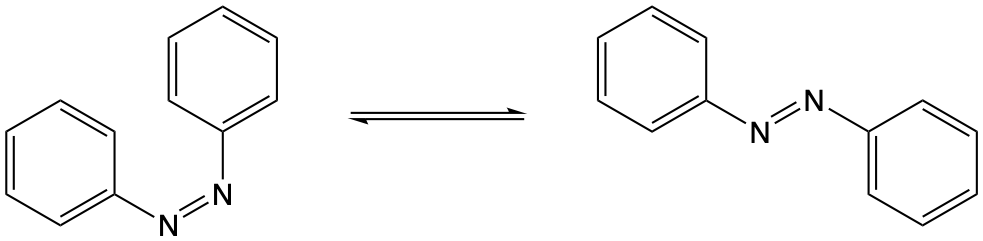
\includegraphics[width=0.7\linewidth]{images/cistransazobenzene} 

}

\caption{The cis-trans isomerisation of azobenzene}\label{fig:cistransazobenzene}
\end{figure}

\begin{itemize}
\item
  Why would you expect the absorption spectrum of each isomer to be different?
\item
  Suggest why the trans conformation is more stable than the cis isomer.
\item
  Use the following data to predict the proportion of each isomer under 360 nm excitation.
\end{itemize}

\begin{longtable}[]{@{}lll@{}}
\caption{\label{tab:azobenzeneabs} The molar extinction coefficient of the two isomers of azobenzene.}\tabularnewline
\toprule
& ε\textsubscript{360} / M\textsuperscript{−1} cm\textsuperscript{−1} & ε\textsubscript{460} / M\textsuperscript{−1} cm\textsuperscript{−1}\tabularnewline
\midrule
\endfirsthead
\toprule
& ε\textsubscript{360} / M\textsuperscript{−1} cm\textsuperscript{−1} & ε\textsubscript{460} / M\textsuperscript{−1} cm\textsuperscript{−1}\tabularnewline
\midrule
\endhead
trans-azobenzene & 22000 & 4500\tabularnewline
cis-azobenzene & 2100 & 5500\tabularnewline
\bottomrule
\end{longtable}

\begin{itemize}
\item
  Would there be more or less trans azobenzene at 460 nm? Justify your answer.
\item
  It has been suggested the 360 nm absorption is an S\textsubscript{0} → S\textsubscript{2} absorption, and the 460 nm band is an S\textsubscript{0} → S\textsubscript{1} absorption. Suggest which energy levels are involved for each of the two transitions and compare it to stilbene which has a similar structure, but the cis and trans absorptions are 280 \& 295 nm respectively.
\end{itemize}

\begin{figure}

{\centering 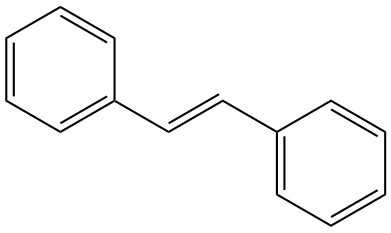
\includegraphics[width=0.3\linewidth]{images/stilbene} 

}

\caption{The  structure of stilbene}\label{fig:stilbene}
\end{figure}

\emph{(This will be a discussion question - please feel free to raise a hand or write comments in the zoom chat. I don't expect to finish this question but hope to get far enough through that a good attempt can be made at home after the LOIL)}

\hypertarget{ch:Workshop2}{%
\chapter{Workshop Questions for Week 2}\label{ch:Workshop2}}

\hypertarget{sec:YieldLifetime}{%
\section{Short mathematical question - Quantum Yield and lifetime}\label{sec:YieldLifetime}}

The quantum yield and lifetime of a dye were measured to be 0.43 \& 2.6 ns respectively. What is the natural lifetime?

\emph{(I will use MCQs and UniDoodle to ask this in class)}

\hypertarget{sec:otherprocesses}{%
\section{Short conceptual question - Effect of other processes}\label{sec:otherprocesses}}

For a given value of τ\textsubscript{0} what happens to the lifetime and quantum yield as k\textsubscript{IC} and k\textsubscript{ISC} increases?

\emph{(This will be a discussion question - please feel free to raise a hand or write comments in the zoom chat)}

\hypertarget{sec:structure}{%
\section{Conceptual question - Effect of structure}\label{sec:structure}}

Fluorescein (figure \ref{fig:fluorescein}) in basic aqueous solution has a quantum yield of fluorescence, Φ\textsubscript{f}, of 0.95, and fluorescence lifetime, τ\textsubscript{f}, of 4.1 ns.

\begin{figure}

{\centering 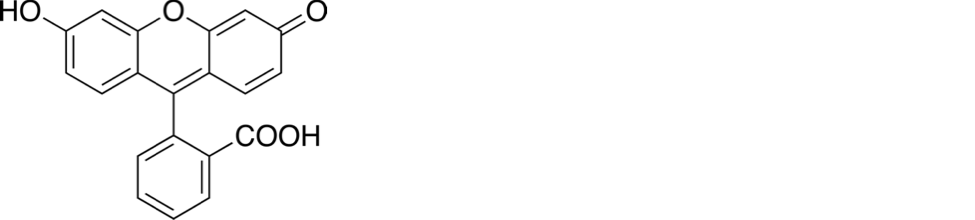
\includegraphics[width=0.7\linewidth]{images/fluorescein} 

}

\caption{The structure of the fluorescent molecule fluorescein}\label{fig:fluorescein}
\end{figure}

\emph{(This will be a discussion question - please feel free to raise a hand or write comments in the zoom chat)}

\hypertarget{conceptual-question---lack-of-symmetry-in-spectra.}{%
\section{Conceptual question - lack of symmetry in spectra.}\label{conceptual-question---lack-of-symmetry-in-spectra.}}

The absorption and emission spectrum of fluorescein is shown in figure (\ref{fig:fluoresceinspec})

\begin{figure}

{\centering 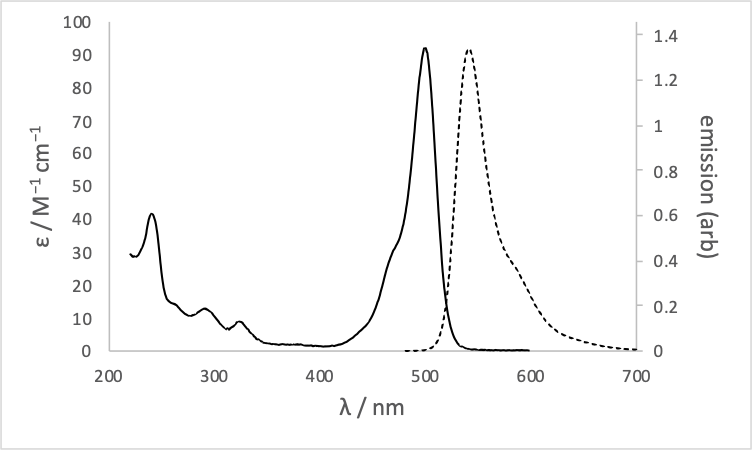
\includegraphics[width=0.7\linewidth]{images/fluoresceinspec} 

}

\caption{The absorption (solid) and emission (dashed) spectrum of fluorescein in basic ethanol.}\label{fig:fluoresceinspec}
\end{figure}

Why are the absorption bands between 200 -- 350 nm not reflected in the emission spectrum?

\hypertarget{sec:stokes}{%
\section{Conceptual question - Stokes' shift}\label{sec:stokes}}

The inorganic dye {[}Ru(bpy)\textsubscript{3}{]}\textsuperscript{2+} has a measured lifetime in water of 580 ns and a natural lifetime of 13.8 µs. The spectrum is shown in figure \ref{fig:Rubpyspec}. What is the origin of the large Stokes' shift in this system?

\begin{figure}

{\centering 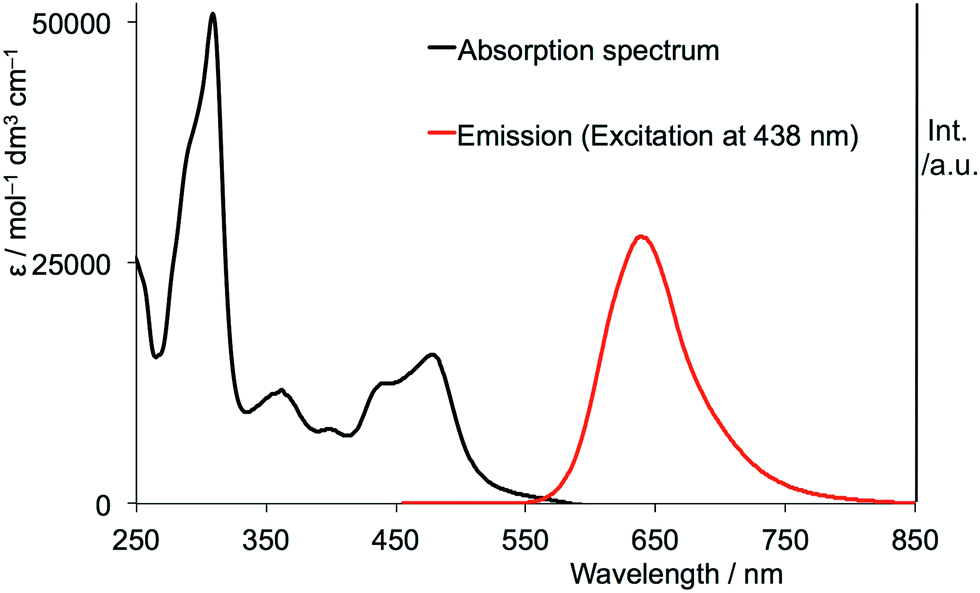
\includegraphics[width=0.7\linewidth]{images/Rubpy3spectra} 

}

\caption{The absorption (black) and emission (red) spectrum of ruthenium tris bypyridine in water.}\label{fig:Rubpyspec}
\end{figure}

Data from Shi \emph{et al.}, Synthesis and characterization of phosphorescent two coordinate copper(I) complexes bearing diamidocarbene ligands. \href{https://doi.org/10.1039/C6DT04016K}{Dalton Trans., 2017,46, 745-752.}

\hypertarget{sec:binding}{%
\section{Conceptual question - the effect of binding on emission}\label{sec:binding}}

The asymmetric cyanine dye YO-Pro-1 is a DNA stain because it has a large increase on fluorescence emission when binding to DNA. The lifetime in free solution is around 2 ps and when bound to DNA is 2.4 ns. What is the structural origin of the large increase of emission upon binding?

\begin{figure}

{\centering 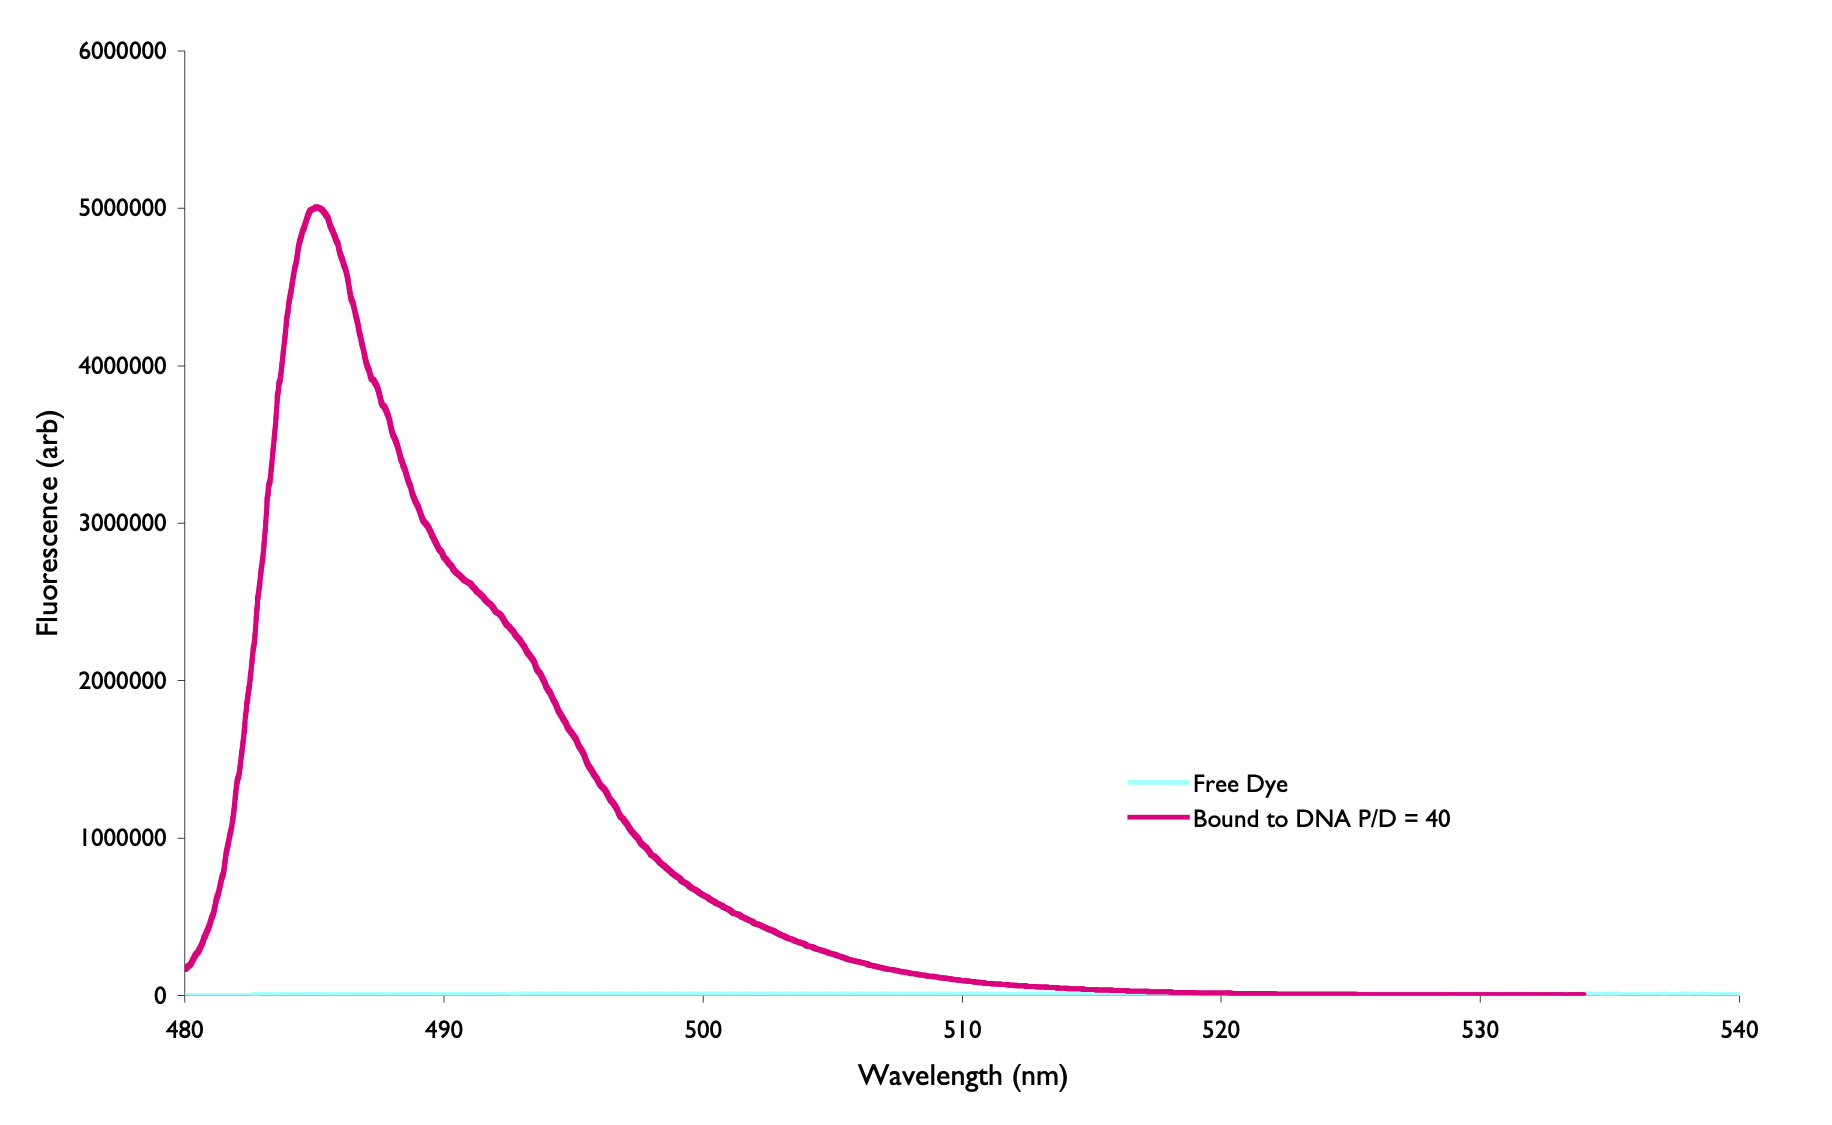
\includegraphics[width=0.7\linewidth]{images/YODNA} 

}

\caption{The emission spectrum of the choromophore YO-Pro-1 when free in aqueous solution (blue) and when bound to DNA (pink)}\label{fig:YODNA}
\end{figure}

\emph{(This will be a discussion question - please feel free to raise a hand or write comments in the zoom chat)}

\hypertarget{extended-question---properties-of-ethidium-bromide-example-exam-question}{%
\section{Extended question - Properties of Ethidium Bromide (Example Exam Question)}\label{extended-question---properties-of-ethidium-bromide-example-exam-question}}

Ethidium bromide (EB, figure \ref{fig:ethidiumstructure} is used as a DNA stain, which is essentially non-fluorescent in aqueous solution, but shows a strong enhancement of emission upon binding to double stranded DNA (which has a negatively charged backbone).

Emission is almost exclusively from the singlet excited state, but a triplet state has been shown to exist, which emits with a low quantum yield (Φ\textsubscript{P} = 0.00006).

\begin{figure}

{\centering 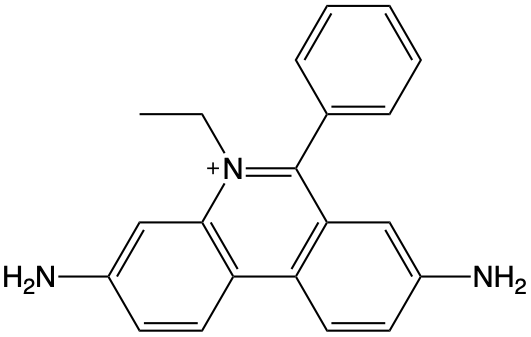
\includegraphics[width=0.3\linewidth]{images/ethidiumstructure} 

}

\caption{The structure of the cationic ethidium bromide chromophore.}\label{fig:ethidiumstructure}
\end{figure}

\begin{itemize}
\item
  Sketch a Jablonski diagram for the processes you know to occur.
\item
  The molar extinction coefficient, ε, of EB has be measured to be 78500 M\textsuperscript{−1} cm\textsuperscript{−1}. What factors contribute to EB having such a high extinction coefficient?
\end{itemize}

The following spectra, lifetimes and quantum yield have been measured for EB in different free solution and DNA systems:

\begin{longtable}[]{@{}lll@{}}
\caption{\label{tab:ethidiumlifetime} The lifetimes and quantum yields of ethidium bromide in aquous solution and when bound to DNA in protiated and deuterated systems.}\tabularnewline
\toprule
& τ / ns & Φ\textsubscript{f}\tabularnewline
\midrule
\endfirsthead
\toprule
& τ / ns & Φ\textsubscript{f}\tabularnewline
\midrule
\endhead
H\textsubscript{2}O (no DNA) & 1.6 & 0.012\tabularnewline
D\textsubscript{2}O (no DNA) & 6.3 &\tabularnewline
DNA & 28.3 & 0.220\tabularnewline
DNA (deuterated) & 38.4 &\tabularnewline
\bottomrule
\end{longtable}

\begin{figure}

{\centering 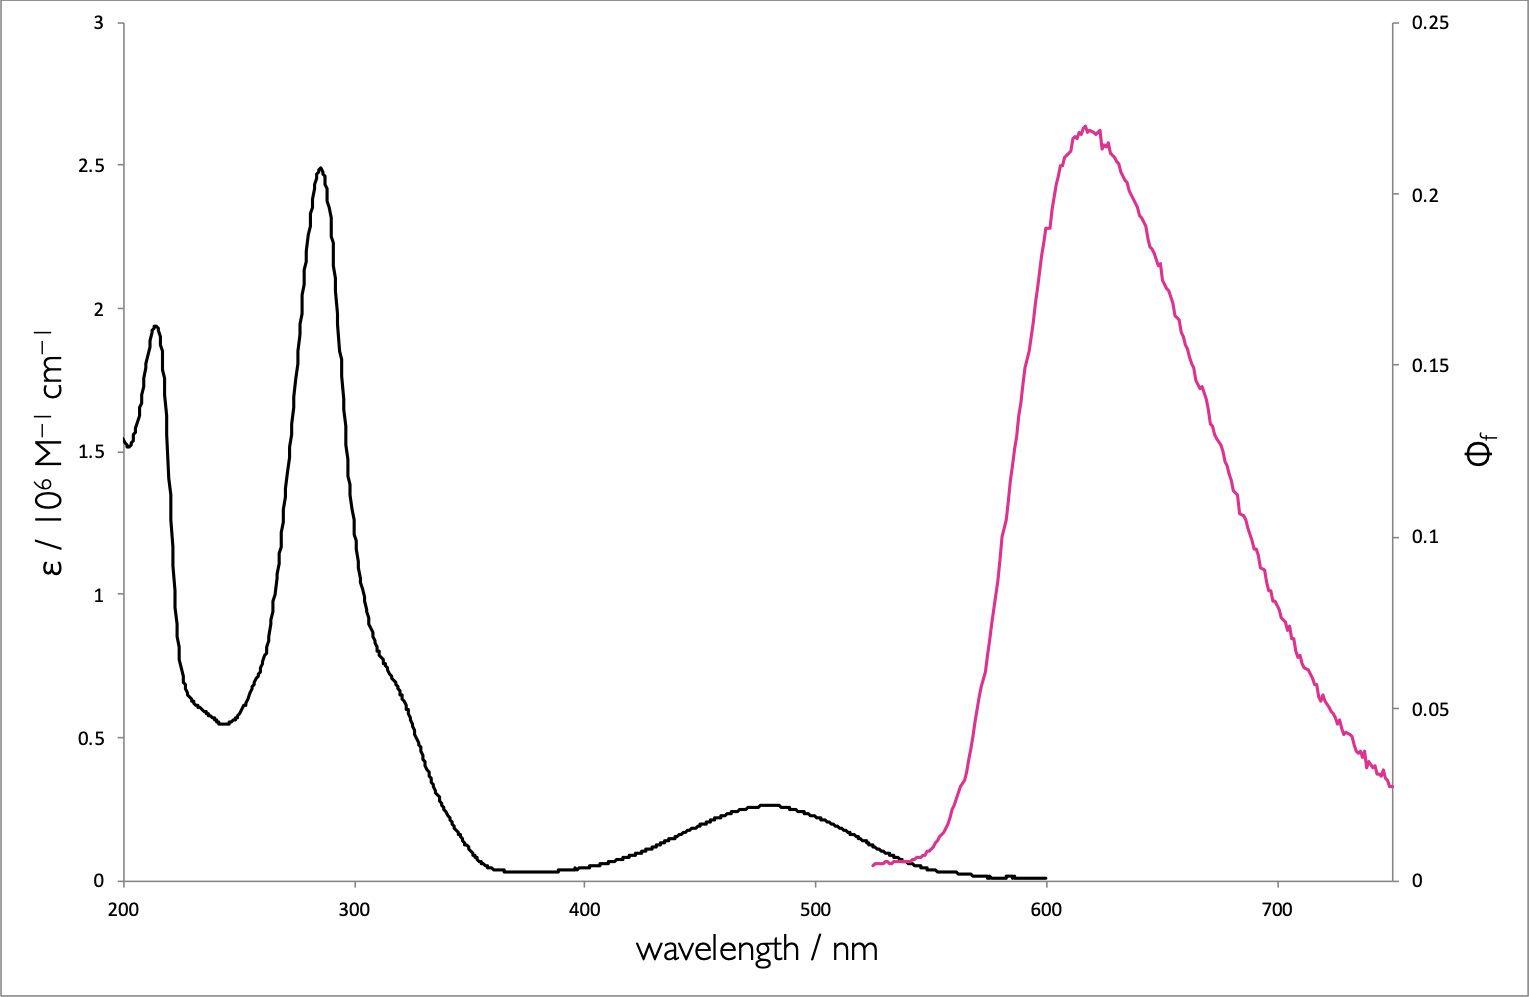
\includegraphics[width=0.3\linewidth]{images/ethidiumspectra} 

}

\caption{The absorption (black) and emission (pink) spectrum of ethidium bromide when bound to DNA.}\label{fig:ethidiumspectra}
\end{figure}

\begin{itemize}
\item
  What factors likely lead to an enhancement of fluorescence quantum yield upon binding to DNA?
\item
  Show that the natural lifetime of EB is 129 ns.
\item
  What is the origin of the large Stoke's shift (λ\textasciitilde max ex\textasciitilde{} = 520 nm, λ\textasciitilde max em\textasciitilde{} = 608 nm)
\item
  What transitions are responsible for the absorption features in the:
  * 400-600 nm range
  * 200-350 nm range
\item
  Why are the features in the 200-350 nm range not replicated in the emission spectrum?
\item
  Why does deuterating the solvent (or DNA) effect the lifetime of the excited state?
\item
  What effect would freezing the samples have on the lifetime, fluorescence quantum yield \& phosphorescence quantum yield.
\end{itemize}

A study of the thermodynamics of the dye DNA system measured the binding constant of EB with DNA to be 1.05 × 10\textsuperscript{6}.

\begin{itemize}
\item
  Why is the measured quantum yield for a system containing 2 µM EB and 20 mM DNA only 0.18?
\item
  Why would increasing the ionic strength of the solution, increase the fluorescence intensity of EB in solution with DNA?
\end{itemize}

\hypertarget{ch:Workshop3}{%
\chapter{Workshop Questions for Week 3}\label{ch:Workshop3}}

\hypertarget{sec:overlap}{%
\section{Short conceptual question - Electronic-vibrational overlap integrals}\label{sec:overlap}}

\begin{figure}

{\centering 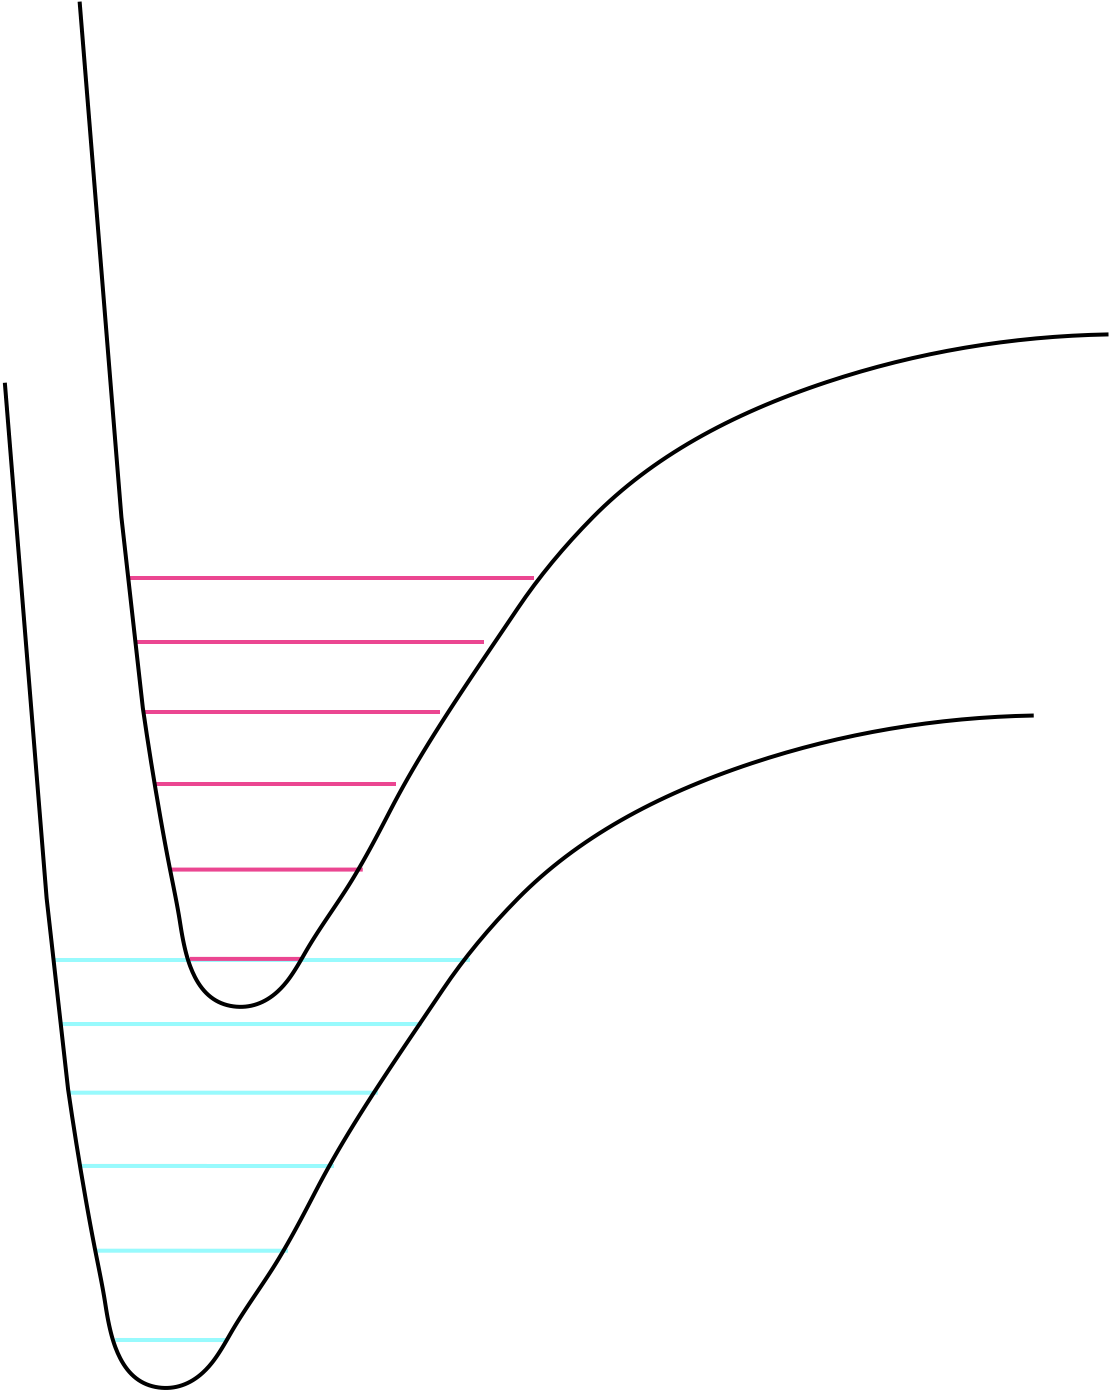
\includegraphics[width=0.7\linewidth]{images/overlap} 

}

\caption{The grond and excited state potential wells and the vibrational levels within them.}\label{fig:overlap}
\end{figure}

On the figure sketch the vibrational energy levels in the ground and the excited state.

How would the following affect this overlap integral?
1. Energy gap.
1. The vibrational energy gaps
1. Reaction coordinate (the difference in structure between ground and excited state)

\emph{(I will use drawing in UniDoodle to ask this in class, with the second part being a discussion question)}

\hypertarget{sec:structureQY}{%
\section{Short conceptual question - The effect of structural changes on quantum yield}\label{sec:structureQY}}

5,10-dihydroindeno{[}2,1-a{]}indene and trans-stilbene (figure \ref{fig:stilbeneindene}) are similar in structure but have very different fluorescent quantum yields of 1.00 and 0.05 respectively, however for trans-stilbene this increases to 0.75 at 77 K. Suggest a reason for the difference in quantum yield of:
- the two molecules
- the two temperatures

\begin{figure}

{\centering 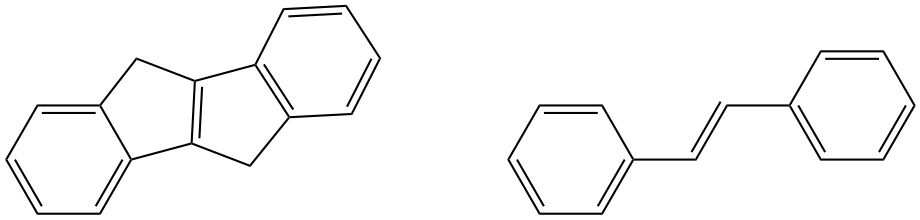
\includegraphics[width=0.6\linewidth]{Images/stilbeneindene} 

}

\caption{5,10-dihydroindeno[2,1-a]indene (left) and trans-stilbene (right)}\label{fig:stilbeneindene}
\end{figure}

\emph{(This will be a discussion question - please feel free to raise a hand or write comments in the zoom chat)}

\hypertarget{sec:ratephos}{%
\section{Short mathematical question - Effect of the rate of singlet triplet intersystem crossing on th quantum yield of phosphorescence}\label{sec:ratephos}}

Why is it likely that the quantum yield of phosphorescence of a sample would increase after the sample is frozen.

\emph{(This will be a discussion question - please feel free to raise a hand or write comments in the zoom chat)}

\hypertarget{sec:calcphos}{%
\section{Short mathematical question - Determining the quantum yield of phosphorescence}\label{sec:calcphos}}

A molecule decays by a combination of internal conversion, intersystem crossing and phosphorescence. What is the quantum yield of phosphorescence?

\begin{itemize}
\tightlist
\item
  k\textsubscript{IC} = 2.1 × 10\textsuperscript{11} s\textsuperscript{−1}
\item
  k\textsubscript{ST} = 2.9 × 10\textsuperscript{9} s\textsuperscript{−1}
\item
  k\textsubscript{TS} = 7.4 × 10\textsuperscript{6} s\textsuperscript{−1}
\item
  k\textsubscript{p}\textsuperscript{o} = 6.2 × 10\textsuperscript{8} s\textsuperscript{−1}
\end{itemize}

\emph{(This will be a discussion question - please feel free to raise a hand or write comments in the zoom chat)}

\hypertarget{sec:exhydrocarbons}{%
\section{Short conceptual question - Deactivation of excited state aromatic hydrocarbsons}\label{sec:exhydrocarbons}}

\begin{longtable}[]{@{}llll@{}}
\caption{\label{tab:smallmolQY} The quantum yields of various deactivation processes in small organic molecules measured at 77 K in a glass matrix.}\tabularnewline
\toprule
& Φ\textsubscript{f} & Φ\textsubscript{ST} & ΔE / kJ mol\textsuperscript{−1}\tabularnewline
\midrule
\endfirsthead
\toprule
& Φ\textsubscript{f} & Φ\textsubscript{ST} & ΔE / kJ mol\textsuperscript{−1}\tabularnewline
\midrule
\endhead
Napthalene & 0.20 & 0.80 & 385\tabularnewline
Anthracene & 0.70 & 0.30 & 318\tabularnewline
Pyrene & 0.6 & low & 322\tabularnewline
Tetracene & 0.1 & 0.65 & 251\tabularnewline
Pentacene & 0.10 & 0.15 & 209\tabularnewline
\bottomrule
\end{longtable}

When examining the data above suggest why it is likely why the quantum yields of both fluorescence and singlet to triplet intersystem crossing decrease with increasing molecule size.

\emph{(This will be a discussion question - please feel free to raise a hand or write comments in the zoom chat)}

\hypertarget{sec:dsolvent}{%
\section{Short conceptual question - Affect of deuteration of solvents.}\label{sec:dsolvent}}

Singlet oxygen has a phosphorescence wavelength of around 1070 nm and a lifetime of 2 µs in water, how would you expect this lifetime to change for singlet oxygen in D\textsubscript{2}O?

\emph{(This will be a discussion question - please feel free to raise a hand or write comments in the zoom chat)}

\hypertarget{sec:isotope}{%
\section{Short conceptual question - Isotope effects on deactivation of an excited state}\label{sec:isotope}}

The fluorescence quantum yield and singlet state lifetime of both proteated and deuterated pyrene are 0.90 and 450 ns respectively. Why does deuteration of the sample have no measureable affect on these values?

Conversely for naphthalene phosphorescence (in glass at 77 K) the quantum yield of phosphoresce increases from 0.05 to \textasciitilde0.80 on deuteration of the sample. (ΔE = 251 kJ mol\textsuperscript{−1} ). Explain this observation with respect to the energy gap law.

\emph{(This will be a discussion question - please feel free to raise a hand or write comments in the zoom chat)}

\hypertarget{sec:heavy}{%
\section{Short conceptual question - The effect of heavy attoms on the rate of intersystem crossing}\label{sec:heavy}}

\begin{longtable}[]{@{}llll@{}}
\caption{\label{tab:heavyatom} The affect of substitution of different halogens on the rates of phosphorescence and singlet to triplet intersystem crossing.}\tabularnewline
\toprule
& k\textsubscript{p} & k\textsubscript{ST} & Φ\textsubscript{p} / Φ \textsubscript{f}\tabularnewline
\midrule
\endfirsthead
\toprule
& k\textsubscript{p} & k\textsubscript{ST} & Φ\textsubscript{p} / Φ \textsubscript{f}\tabularnewline
\midrule
\endhead
Napthalene & 0.05 & 0.39 & 0.09\tabularnewline
1-fluoronaphthalene & 0.23 & 0.42 & 0.07\tabularnewline
1-chloronaphthalene & 1.1 & 2.35 & 5.2\tabularnewline
1-bromonaphthalene & 13.5 & 36.5 & 169\tabularnewline
1-iodonaphthalene & 190 & 310 & \textgreater760\tabularnewline
\bottomrule
\end{longtable}

Briefly explain why the rates of these processes increase as we move down the group.

\emph{(This will be a discussion question - please feel free to raise a hand or write comments in the zoom chat)}

\hypertarget{sec:osphen}{%
\section{Short conceptual question - The effect of absorbance and emission wavelengths on the quantum yield of emission}\label{sec:osphen}}

\begin{longtable}[]{@{}llllll@{}}
\caption{\label{tab:osphen} The spectroscopic details of a family of osmium complexes.}\tabularnewline
\toprule
& λ\textsubscript{abs} / nm & λ\textsubscript{em} / nm & ΔE / eV & τ/ ns & Φ\textsubscript{em}\tabularnewline
\midrule
\endfirsthead
\toprule
& λ\textsubscript{abs} / nm & λ\textsubscript{em} / nm & ΔE / eV & τ/ ns & Φ\textsubscript{em}\tabularnewline
\midrule
\endhead
{[}Os(phen)\textsubscript{3}{]}\textsuperscript{2+} & 650 & 720 & 0.186 & 260 & 0.016\tabularnewline
{[}Os(phen)\textsubscript{2}(dppene){]}\textsuperscript{2+} & 455 & 609 & 0.69 & 1830 & 0.138\tabularnewline
{[}Os(phen)(dppene)\textsubscript{2}{]}\textsuperscript{2+} & 400 & 530 & 0.761 & 3600 & 0.518\tabularnewline
\bottomrule
\end{longtable}

Why does the fluorescence lifetime increase as the phenanthroline ligands are replaced with dppene ligands?

\emph{(This will be a discussion question - please feel free to raise a hand or write comments in the zoom chat)}

\hypertarget{ch:Workshop4}{%
\chapter{Workshop Questions for Week 4}\label{ch:Workshop4}}

\hypertarget{sec:diffcontrol}{%
\section{Short mathematical question - Determining rates of diffusion controlled quenching}\label{sec:diffcontrol}}

The rate of diffusion (\(k_d\)) in solution is given by equation \eqref{eq:diffcontrolrate}, where \(\eta\) is the viscosity of the solution.

\begin{equation}
k_d = \frac{8RT}{3 \eta}
\label{eq:diffcontrolrate}
\end{equation}

Determine the maximum possible rate of diffusion controlled quenching at 20 ºC in:

\begin{enumerate}
\def\labelenumi{\alph{enumi}.}
\tightlist
\item
  water (\(\eta=\) 1.0016 mPa s)
\item
  methanol (\(\eta=\) 0.594 mPa s)
\end{enumerate}

\emph{(I will use UniDoodle to ask this in class - please attempt before the LOIL)}

\hypertarget{sec:emintquench}{%
\section{Short mathematical question - Determining the effect of diffusion controlled quenching on emission intensity}\label{sec:emintquench}}

What emisison intensity would you expect if 50 mM of a quencher quenches the emission of a chromophore dissolved in basic ethanol at 10 ºC, with natural lifetime of 13.2 ns and emission quantum yield, Φ\textsubscript{f}, of 0.32, if the unqunched intensity is 35240.

\(\eta\)\textasciitilde EtOH, 10 ºC\textasciitilde{} = 1.394 mPa s

\emph{(This will be a discussion question - please attempt before the LOIL and be ready to contribute to the maths process)}

\hypertarget{sec:temp}{%
\section{Short conceptual question - effect of temperature}\label{sec:temp}}

YO-Pro-1 is quenched in the presence of molecular oxygen, as the temperature increases this quenching increases, what does this indicate about the mechanism of quenchign and why?

\emph{(This will be a discussion question - please feel free to raise a hand or write comments in the zoom chat)}

\hypertarget{sec:static}{%
\section{Short conceptual question - static quenching}\label{sec:static}}

When in the presence of a quencher the intensity of emission of a chromophore (τ\textsubscript{0} = 5.2 ns) was reduced from 4200 cps to 2100 cps at 25 ºC and 1800 cps at 10 ºC. What would the lifetime of the quenched chromophore be at 25 ºC?

\emph{(This will be a discussion question - please feel free to raise a hand or write comments in the zoom chat)}

\hypertarget{sec:static2}{%
\section{Short conceptual question - static quenching}\label{sec:static2}}

10-methylacridinium chloride (MAC) is quenced in the presence of adenosine monophosphate (AMP, figure (\ref{fig:AMP})). The effect of quenching is enhanced by addition of sodium sulfate.

In a separate experiment the emssion of MAC is unaffected by addition of sodium sulfate (when not in the presence of AMP).

Suggest the mechanism of quenching, justifying this with reference to the experimental data.

\begin{figure}

{\centering 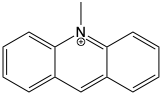
\includegraphics[width=0.3\linewidth]{images/MAC} 

}

\caption{The structure of methyl acridinium.}\label{fig:MAC}
\end{figure}

\begin{figure}

{\centering 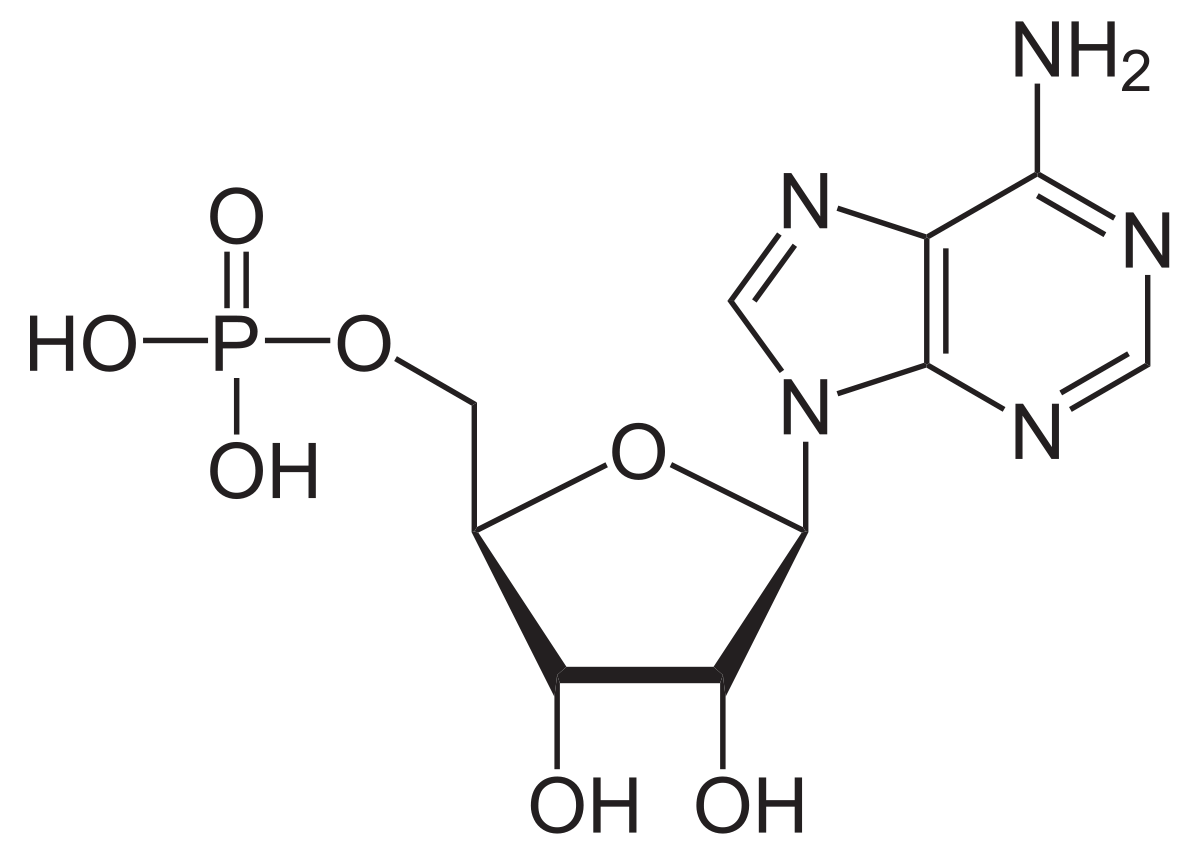
\includegraphics[width=0.3\linewidth]{images/AMP} 

}

\caption{The structure of adenosine monophosphate.}\label{fig:AMP}
\end{figure}

\emph{(This will be a discussion question - please feel free to raise a hand or write comments in the zoom chat)}

\hypertarget{sec:acridone}{%
\section{Long mathematical question - Quenching of emission of acridone}\label{sec:acridone}}

Acridone (figure \ref{fig:acridone})is found to be quenched in the presence of potassium iodide in aqueous solution at 26 oC. Solutions were maintained at constant ionic strength by use of KNO2, the KNO2 does not affect the emission intensity of the solution.

\begin{figure}

{\centering 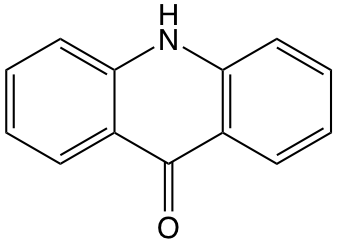
\includegraphics[width=0.3\linewidth]{images/acridone} 

}

\caption{The structure of acridone.}\label{fig:acridone}
\end{figure}

The following data were collected for the emission of acridone.

\begin{longtable}[]{@{}cccc@{}}
\caption{\label{tab:acridonequench} The effect of potassium iodide concentration on emission intensity and fluorescence lifetime of acridone in aqueous solution.}\tabularnewline
\toprule
{[}KI{]} / M & {[}KNO\textsubscript{2}{]} / M & Emission intensity / arb & τ / ns\tabularnewline
\midrule
\endfirsthead
\toprule
{[}KI{]} / M & {[}KNO\textsubscript{2}{]} / M & Emission intensity / arb & τ / ns\tabularnewline
\midrule
\endhead
0 & 1.100 & 16580 & 17.60\tabularnewline
0.040 & 1.060 & 3753 & 3.90\tabularnewline
0.100 & 1.000 & 1566 & 1.80\tabularnewline
0.200 & 0.900 & 721 & 0.95\tabularnewline
0.300 & 0.800 & 446 & 0.64\tabularnewline
0.500 & 0.600 & 242 & 0.39\tabularnewline
0.800 & 0.300 & 121 & 0.25\tabularnewline
\bottomrule
\end{longtable}

\begin{enumerate}
\def\labelenumi{\arabic{enumi}.}
\item
  Using an appropriate plot (or plots) determine if the quenching is static, dynamic or a combination of both mechanisms.
\item
  Determine any relevant quenching constants (k\textsubscript{d} and/or K\textsubscript{S} )
\end{enumerate}

\emph{(This will be a discussion question - please be ready to contribute to the maths process)}

\hypertarget{ch:Workshop5}{%
\chapter{Workshop Questions for Week 5}\label{ch:Workshop5}}

\hypertarget{sec:O2quench}{%
\section{Short conceptual question - O2 quenching}\label{sec:O2quench}}

\begin{enumerate}
\def\labelenumi{\arabic{enumi}.}
\item
  Given molecular oxygen has an emission with λ\textsubscript{max} around 1280 nm why is it such a good quencher of excited states?
\item
  Why is the efficiency of quenching lower for excited singlet states?
\end{enumerate}

\emph{Are you all happy with the energy level diagram of molecular oxygen?}

\emph{(This will be a discussion question - please feel free to raise a hand or write comments in the zoom chat)}

\hypertarget{sec:FRET}{%
\section{Short mathematical question - Förster resonance energy transfer}\label{sec:FRET}}

A donor, D, with an unquenched lifetime of 5.0 ns, was found to have a steady state emission intensity of 20.5 in free solution and 4.1 when in the presence of a quencher, Q. Assuming the Förster distance is 50 Å determine :

\begin{enumerate}
\def\labelenumi{\arabic{enumi}.}
\tightlist
\item
  the transfer efficiency, E.
\item
  the lifetime of D in the presence of the quencher Q
\item
  the equilibrium separation of D \& Q
\item
  the rate constant for energy transfer
\end{enumerate}

\emph{(This will be a discussion question - please feel free to raise a hand or write comments in the zoom chat)}

\hypertarget{sec:FRETdist}{%
\section{Short conceptual quesiton - Förster distance}\label{sec:FRETdist}}

Determine the quantum yield of emission of the donor in a FRET pair system where donor and acceptor are separated by the Förster distance, the lifetime of the unquenched system is 8.4 ns. The unquenched quantum yield is 0.58*

\emph{(I will poll this question on UniDoodle and then maybe discuss some of the responses)}

\hypertarget{sec:donoracceptor}{%
\section{Short conceptual quesiton - Donor-accceptor system}\label{sec:donoracceptor}}

In a single molecule study of a donor bound to an acceptor via a flexible, short aliphatic chain it was found that lifetime of the excited state varied (time beween single photon detection of emission after an excitation pulse). Suggest why this is the case.

\emph{(This will be a discussion question - please feel free to raise a hand or write comments in the zoom chat)}

\hypertarget{sec:ruquench}{%
\section{Short conceptual quesiton - Quenching of ruthenium}\label{sec:ruquench}}

Ruthenium tris bipyridine {[}Ru(bpy)\textsubscript{3}{]}\textsuperscript{2+} has a λ\textasciitilde max, abs\textasciitilde{} = 470 nm and λ\textasciitilde max, em\textasciitilde{} = 465 nm. The natural lifetime is 13.6 µs.

Suggest why molecular oxygen is an efficient quencher of the emmission of {[}Ru(bpy)\textsubscript{3}{]}\textsuperscript{2+}.

\emph{(This will be a discussion question - please feel free to raise a hand or write comments in the zoom chat)}

\hypertarget{ch:Workshop6}{%
\chapter{Workshop Questions for Week 6}\label{ch:Workshop6}}

\hypertarget{short-conceptual-question---change-in-behaviour-on-freezing}{%
\section{Short conceptual question - change in behaviour on freezing}\label{short-conceptual-question---change-in-behaviour-on-freezing}}

As the concentration of a species increases the wavelength of emission increases in the solution phase but this same shift in wavelength is not when the solution is frozen. What photochemical process may be occuring to explain this effect?

\hypertarget{short-conceptual-question---effect-of-polar-solvents-on-emission}{%
\section{Short conceptual question - effect of polar solvents on emission}\label{short-conceptual-question---effect-of-polar-solvents-on-emission}}

Solutions containing anthracence and diethylaniline are shown to have broad emission at around 450 nm in toluene, but in dichloromethane no emission is observed.

The emission from athracene has λ\textsubscript{max} of 375 nm.

Suggest the processes going on which account for these observations.

\hypertarget{short-conceptual-question---isoemissive-point}{%
\section{Short conceptual question - isoemissive point}\label{short-conceptual-question---isoemissive-point}}

As the concentration of pyrene dissolved in toluene increases a new broad band with a broad featureless spectrum is observed, which is from excimer emisison. What evidence is there that emission is only from single molecule and excimer emission and no other states?

How would the absorption spectrum change as the concentration increases?

\begin{figure}

{\centering 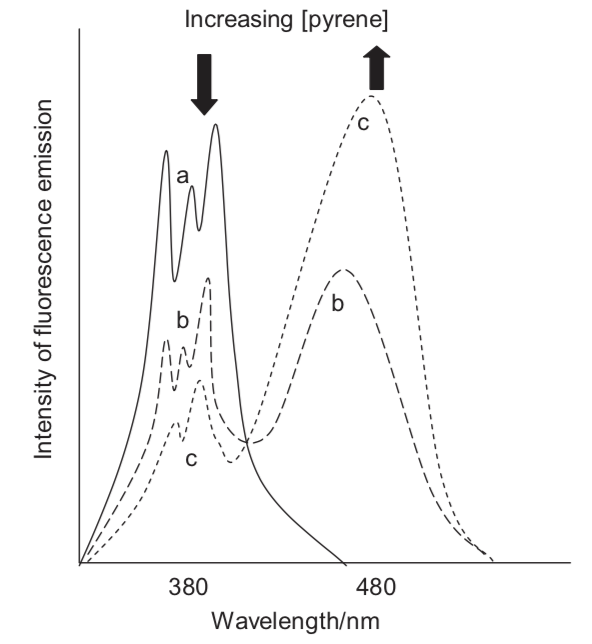
\includegraphics[width=0.3\linewidth]{images/pyrene} 

}

\caption{The emission spectrum of pyrene in tolune as low (solid line) and higher (dotted lines) concentrations.}\label{fig:pyrene}
\end{figure}

\hypertarget{short-conceptual-question---redox-chemistry}{%
\section{Short conceptual question - redox chemistry}\label{short-conceptual-question---redox-chemistry}}

Why does formation of an excited state decrease both the oxidation and reduction potential of a species?

\hypertarget{short-conceptual-question---effect-of-time-delay}{%
\section{Short conceptual question - effect of time delay}\label{short-conceptual-question---effect-of-time-delay}}

If a solution of pyrene in cyclohexane is excited with a very short (ps) pulse of lightafter 1 ns the emission spectrum observed is mainly that of the momomer, whereas after 100 ns emission is principally from the excimer. Why is this the case?

\hypertarget{short-conceptual-question---lifetimes}{%
\section{Short conceptual question - lifetimes}\label{short-conceptual-question---lifetimes}}

The emission spectra of 2-phenylindole shows a marked difference with changes in concentration.

At a concentration of 1 × 10\textsuperscript{−5} M the measured lifetime is 0.86 ns, whereas at 5 × 10\textsuperscript{−3} M the measured lifetime is 3.42 ns.

\begin{figure}

{\centering 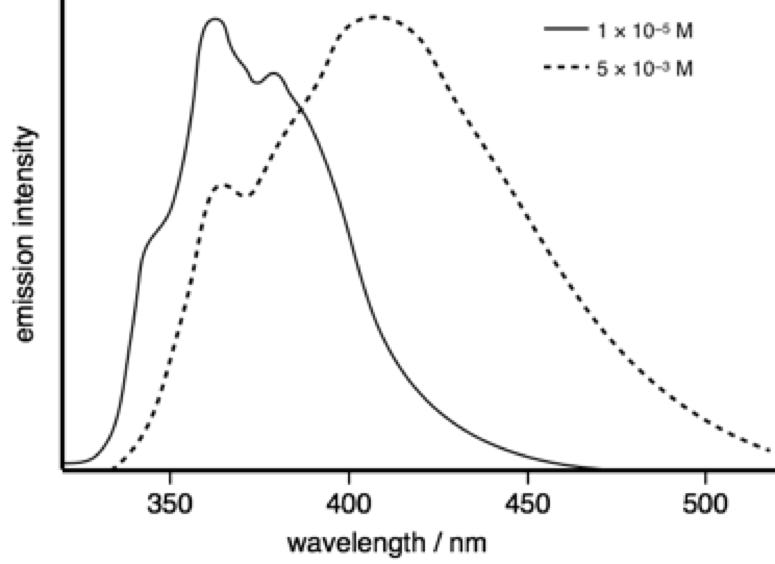
\includegraphics[width=0.3\linewidth]{images/phenylindole} 

}

\caption{The emission spectrum of pyrene in tolune as low (solid line) and higher (dotted lines) concentrations.}\label{fig:phenylindole}
\end{figure}

Why does the measured lifetime depend upon concentration?

  \bibliography{book.bib,packages.bib}

\end{document}
